%----------------------------------------------------------------------------------------
%	PACKAGES AND OTHER DOCUMENT CONFIGURATIONS
%----------------------------------------------------------------------------------------

\documentclass[11pt]{diazessay} % Font size (can be 10pt, 11pt or 12pt)
\usepackage{float}
\usepackage{sectsty}
\usepackage[numbers]{natbib}
\sectionfont{\centering}
\usepackage{listings}
\usepackage{color}

\definecolor{dkgreen}{rgb}{0,0.6,0}
\definecolor{gray}{rgb}{0.5,0.5,0.5}
\definecolor{mauve}{rgb}{0.58,0,0.82}

\lstset{ 
%         language=Matlab,                                % choose the language of the code
%       basicstyle=10pt,                                % the size of the fonts that are used for the code
%         numbers=left,                                   % where to put the line-numbers
%         numberstyle=\footnotesize,                      % the size of the fonts that are used for the line-numbers
%         stepnumber=1,                                           % the step between two line-numbers. If it's 1 each line will be numbered
%         numbersep=5pt,                                  % how far the line-numbers are from the code
%       backgroundcolor=\color{white},          % choose the background color. You must add \usepackage{color}
%         showspaces=false,                               % show spaces adding particular underscores
%         showstringspaces=false,                         % underline spaces within strings
%         showtabs=false,                                         % show tabs within strings adding particular underscores
%       frame=single,                                           % adds a frame around the code
%       tabsize=2,                                              % sets default tabsize to 2 spaces
%       captionpos=b,                                           % sets the caption-position to bottom
         breaklines=true,                                        % sets automatic line breaking
%         breakatwhitespace=false,                        % sets if automatic breaks should only happen at whitespace
%         escapeinside={\%*}{*)}                          % if you want to add a comment within your code
}

\lstset{frame=tb,
  language=php,
  aboveskip=3mm,
  belowskip=3mm,
  showstringspaces=false,
  columns=flexible,
  basicstyle={\small\ttfamily},
  numbers=none,
  numberstyle=\tiny\color{gray},
  keywordstyle=\color{blue},
  commentstyle=\color{dkgreen},
  stringstyle=\color{mauve},
  breaklines=true,
  breakatwhitespace=true,
  tabsize=3
}
%----------------------------------------------------------------------------------------
%	TITLE SECTION
%----------------------------------------------------------------------------------------

\title{\textbf{Traffic Analysis} \\ {\Large\itshape A write-up}} % Title and subtitle

\author{\textbf{Matthew Doherty \& Daniel de la Harpe} \\ \textit{Rhodes University}} % Author and institution

\date{\today} % Date, use \date{} for no date

%----------------------------------------------------------------------------------------

\begin{document}

\maketitle % Print the title section

%----------------------------------------------------------------------------------------
%	ABSTRACT AND KEYWORDS
%----------------------------------------------------------------------------------------

%\renewcommand{\abstractname}{Summary} % Uncomment to change the name of the abstract to something else

\renewcommand{\thesection}{\arabic{section}}
\renewcommand{\thesubsection}{\arabic{subsection}}
\renewcommand{\thesubsubsection}{\arabic{subsubsection}}
\renewcommand{\thesubsection}{\thesection.\arabic{subsection}}
\renewcommand{\thesubsubsection}{\thesubsection.\arabic{subsubsection}}

\vspace{30pt} % Vertical whitespace between the abstract and first section

%----------------------------------------------------------------------------------------
%	ESSAY BODY
%----------------------------------------------------------------------------------------

% "*" means no numbering -> \section*{Introduction}

\section{Introduction}



%------------------------------------------------

\section{Traffic Overview}

\begin{figure}[H]
        \centering
        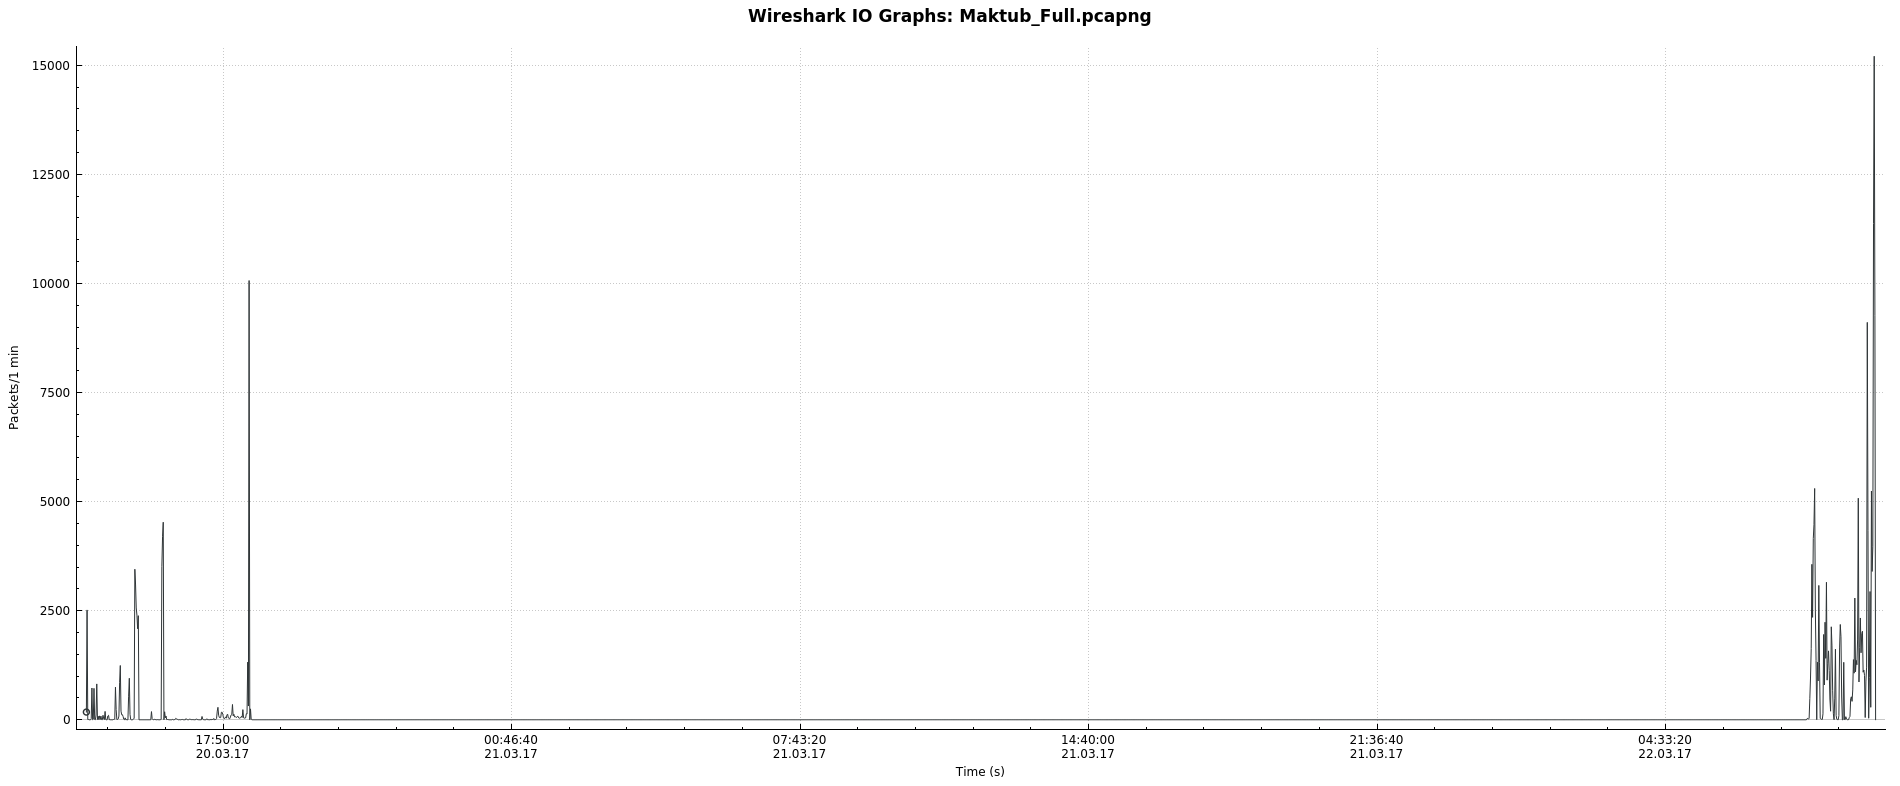
\includegraphics[scale=0.30]{Maktub_Full.png}
    \caption{Pcap Lifetime graph}
\end{figure}

\begin{figure}[H]
        \centering
        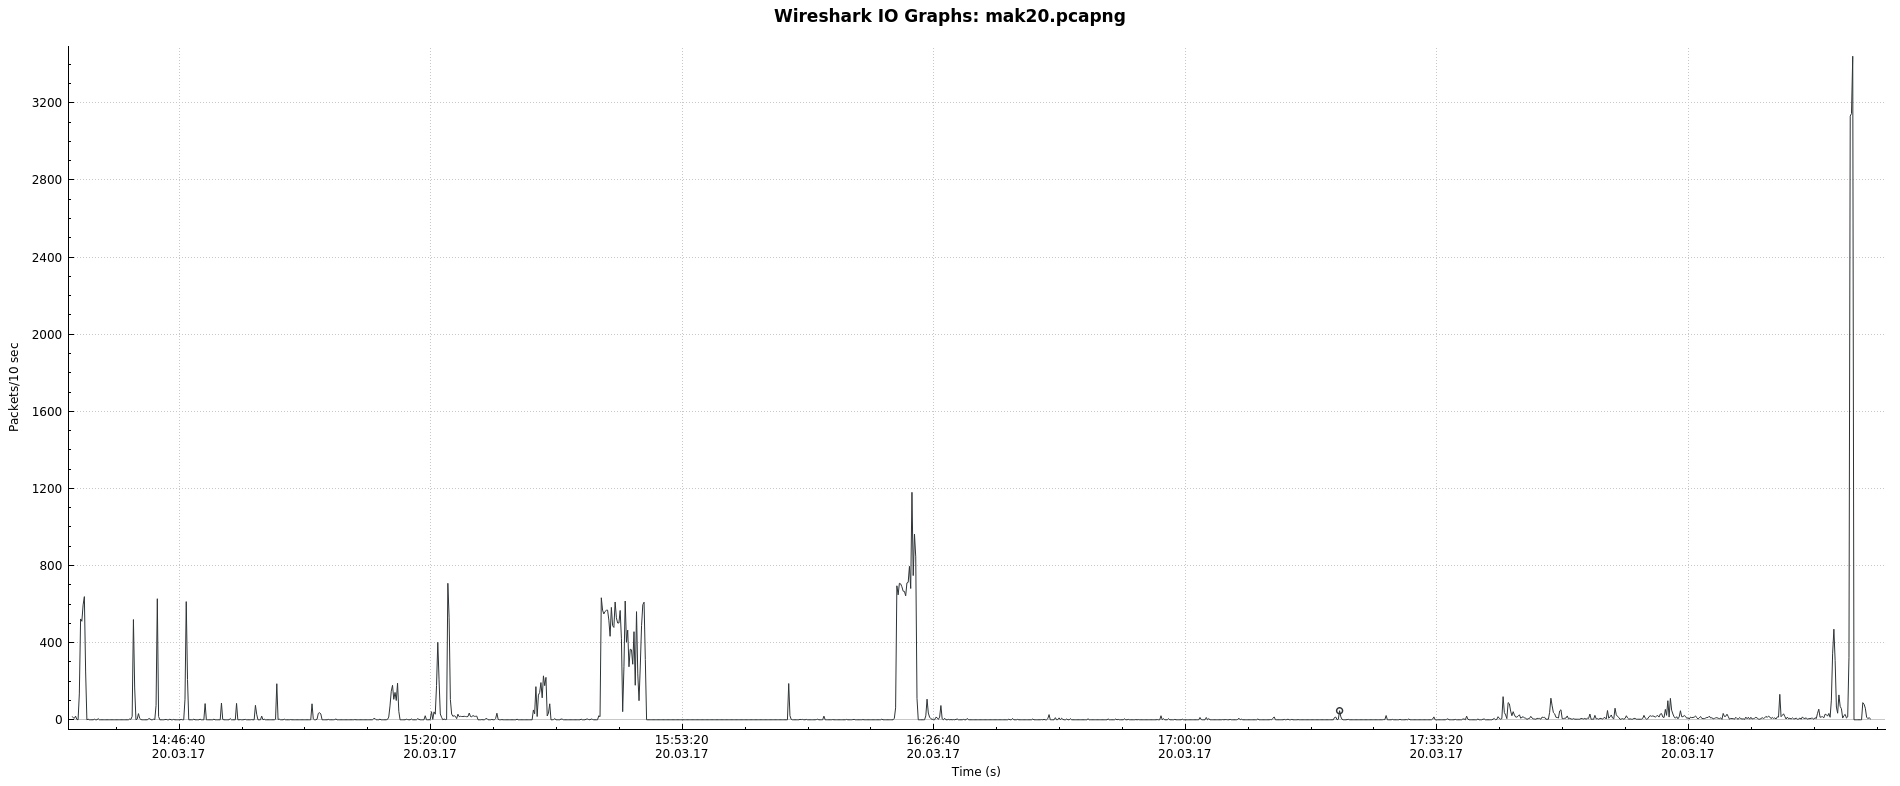
\includegraphics[scale=0.30]{mak20.png}
    \caption{IO graph for 2017-03-20} 
\end{figure}

\begin{figure}[H]
        \centering
        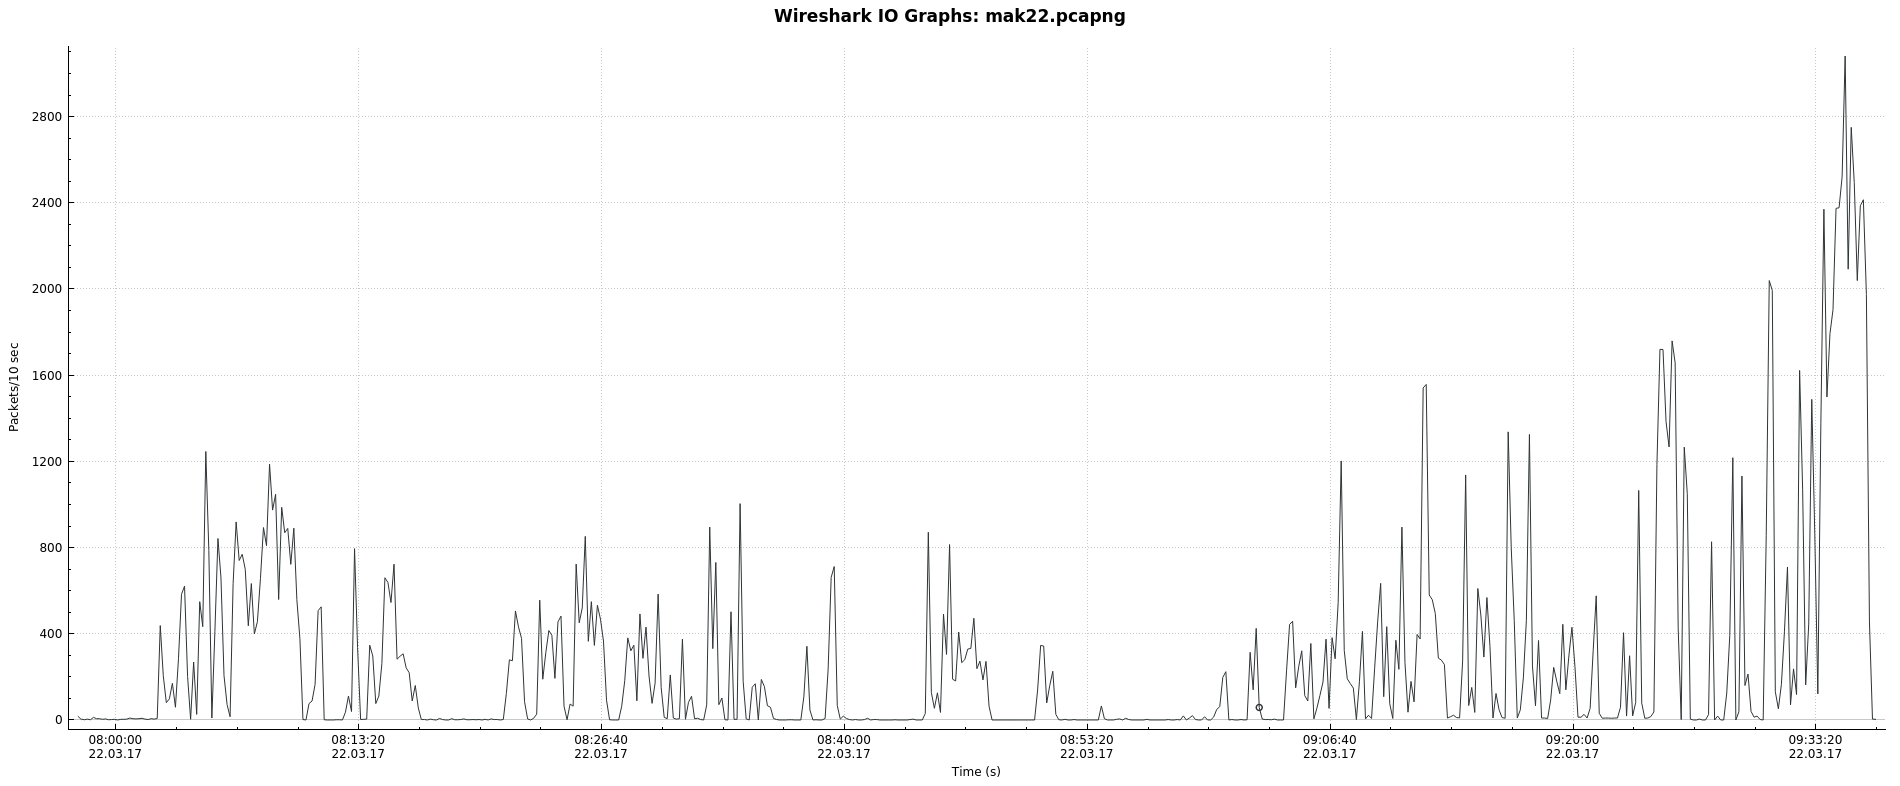
\includegraphics[scale=0.30]{mak22.png}
    \caption{IO Graph for 2017-03-22}
\end{figure}

This analysis examines events that took place on a South African network on the 2017-03-20 and 2017-03-22. We will make the argument, based purely on captured network traffic and inferences gleaned from malware analysis, that a host was compromised with a ransomware variant known as Maktub. 

The three graphs depict packets per 10 seconds for traffic for a full network capture over the entire time period, followed by traffic generated on the 20th and 22nd. The traffic was divided in this way to logically separate the behavior associated with each time sequence. The story of the infected host is encapsulated on the first day whereas the second day exhibits indirect behavior of the ransomware strain as the target machine has been taken offline.  

A point to make about attacks of this kind, is that they can easily slip between the cracks since benign traffic is by far the most dominant communication on the network. Most of the traffic generated involves the target host receiving legitimate windows updates from trusted IP addresses. In monitoring the DNS traffic closely we found some interesting queries for known malicious sites. We set out to uncover the initial execution malicious code and how communication with the C2 (command and control server) was carried out.

Legitmate windows update from Ikai CDN 
DNS for onion domain singapoor 
DNS for cryptostorm to establish VPN Germany
Get Windows-CryptoAPI from comodoca 
China DNS req  for 1.83.255.178 

Cryptostorm VPN connect over TLS 
192.36.27.5 -> Amsterdam IP for onion (Entry node)
103.198.0.2     45jngpxc4cgsxqxc.onion.link -> Singapore

%------------------------------------------------

\section{Traffic for initial compromise}

On the 2017-03-20 our host (10.0.0.5) seems to be engaged in routine Windows updates from IPs associated with Microsoft and Akamai (A legitimate CDN, content distribution network). The first signs of anomalous activity commence. A mail with an attachment, potentially a msword document is fetched after a "503 Backend fetch failed". The destination IP is associated with a onion domain (Host: 45jngpxc4cgsxqxc.onion.link). The .onion domain refers to TOR hidden services which require the TOR browser to interpret the protocol and connect to the hidden service. TOR is a privacy oriented protocol which aims to obscure the origin of the sender, by encapsulating a packet in three layers of encryption prior to routing the packet through three intermediaries nodes before reaching the server. The protocol serves a valuable role to actors of differing motivation. The protocol is not only used by activists and those most vulnerable but also those who exploit it for profit. The ".link" allows for for convenience at the expense of \cite{onionlink}. This allowed the target system to visit a TOR hidden service hosted by our attackers. The onion link confirms our suspicions as it is associated with a malware analysis of an malicious windows executable inserted inside a benign looking update policy word document \cite{hybrid}.


\begin{lstlisting}
2017-03-20 15:20:08.517517 IP (tos 0x0, ttl 128, id 4560, offset 0, flags [DF], proto TCP (6), length 551)
    10.0.0.5.52848 > 103.198.0.2.80: Flags [P.], cksum 0x4696 (correct), seq 1:512, ack 1, win 4236, length 511: HTTP, length: 511
        GET / HTTP/1.1
        Accept: image/jpeg, application/x-ms-application, image/gif, application/xaml+xml, image/pjpeg, application/x-ms-xbap, application/vnd.ms-excel, application/vnd.ms-powerpoint, application/msword, */*
        Accept-Language: en-US
        User-Agent: Mozilla/4.0 (compatible; MSIE 8.0; Windows NT 6.1; Trident/4.0; SLCC2; .NET CLR 2.0.50727; .NET CLR 3.5.30729; .NET CLR 3.0.30729; Media Center PC 6.0; InfoPath.2)
        Accept-Encoding: gzip, deflate
        Host: 45jngpxc4cgsxqxc.onion.link
        Connection: Keep-Alive

E..'..@...u4
...g....p.P*R>....*P...F...GET / HTTP/1.1
Accept: image/jpeg, application/x-ms-application, image/gif, application/xaml+xml, image/pjpeg, application/x-ms-xbap, application/vnd.ms-excel, application/vnd.ms-powerpoint, application/msword, */*
Accept-Language: en-US
User-Agent: Mozilla/4.0 (compatible; MSIE 8.0; Windows NT 6.1; Trident/4.0; SLCC2; .NET CLR 2.0.50727; .NET CLR 3.5.30729; .NET CLR 3.0.30729; Media Center PC 6.0; InfoPath.2)
Accept-Encoding: gzip, deflate
Host: 45jngpxc4cgsxqxc.onion.link
Connection: Keep-Alive

2017-03-20 15:20:08.790039 IP (tos 0x18, ttl 52, id 30272, offset 0, flags [DF], proto TCP (6), length 524)
    103.198.0.2.80 > 10.0.0.5.52848: Flags [P.], cksum 0x6305 (correct), seq 1:485, ack 512, win 123, length 484: HTTP, length: 484
        HTTP/1.1 503 Backend fetch failed
        Date: Mon, 20 Mar 2017 08:21:16 GMT
        Content-Type: text/html; charset=utf-8
        Retry-After: 5
        Age: 0
        X-Cache: MISS
        Content-Length: 286
        Connection: keep-alive

        <!DOCTYPE html>
        <html>
          <head>
            <title>503 Backend fetch failed</title>
          </head>
          <body>
            <h1>Error 503 Backend fetch failed</h1>
            <p>Backend fetch failed</p>
            <h3>Guru Meditation:</h3>
            <p>XID: 288687254</p>
            <hr>
            <p>Varnish cache server</p>
          </body>
        </html>
    103.198.0.2.80 > 10.0.0.5.52849: Flags [P.], cksum 0x7d3d (correct), seq 1:1133, ack 311, win 123, length 1132: HTTP, length: 1132
        HTTP/1.1 500 Internal Server Error
        Content-Length: 856
        Content-Encoding: gzip
        X-Check-Tor: false
        Content-Security-Policy: upgrade-insecure-requests
        X-Onion-Url: 45jngpxc4cgsxqxc.onion
        Date: Mon, 20 Mar 2017 08:21:20 GMT
        Age: 0
        X-Cache: MISS
        Connection: keep-alive

E.....@.4..zg...
....P.q!'(.k.k}P..{}=..HTTP/1.1 500 Internal Server Error
Content-Length: 856
Content-Encoding: gzip
X-Check-Tor: false
Content-Security-Policy: upgrade-insecure-requests
X-Onion-Url: 45jngpxc4cgsxqxc.onion
Date: Mon, 20 Mar 2017 08:21:20 GMT
Age: 0
X-Cache: MISS
Connection: keep-alive

...........U[o.6.~v~....{.........@...k2.1..c..E2$....!\%........|.....Y.[Y\..5......^Bq..V.B=..Rw."J{Rj....k2..Q.....v..}..`............9...,<.(.n.........{..s'.9...?........6.....E;...`O..-........(.4..9el.....p.\.2.9-...n.... s..A.k.|.8.\i....2....3.7|..Z.....-u....+.6.....N?...M.
.n.-2..+.2..*dm......[RJ.\N.B
.Yn.X...D..h......E...-S.jJ..............g...Y.....pb......+....*..k..../I....Q7x.....r\%....NT...l:=.}2..r..[p....5...........?....W..Z....B2.....H..(._JQ>.t...O..s..7..]P"*,.~.....+x{ .~..X..E.k.......S3.........7(LK.wB.D..\..0G.$.2..B.......,...'y.......,H...   .{.|.a....)Tz.^.,.;N<.F[..iDYv...U<hK....Og....3f.oFi....>.
.1{.$.W....CI..bmqJ......2c...S...1...O.._xk......J.......;'.E_qs...../.....S.!...}.}.N!I....c..V..c..o\%.2.R.....D...l...0..m....?.....?}K.X.........ry?`~...........xl...-.....c.:yN   ~......n.36z..n.#|..qn..M..w..t.......


    10.0.0.5.137 > 103.198.0.2.137: [udp sum ok]
>>> NBT UDP PACKET(137): QUERY; REQUEST; BROADCAST
TrnID=0xF66C
OpCode=0
NmFlags=0x1
Rcode=0
QueryCount=1
AnswerCount=0
AuthorityCount=0
AddressRecCount=0
QuestionRecords:
Name=*               NameType=0x00 (Workstation)
QuestionType=0x21
QuestionClass=0x1
\end{lstlisting}
\begin{lstlisting}
00:16:6f:98:80:74 -> c8:51:95:2c:35:73, [udp] 10.0.0.5:61226         -> 10.0.0.2:53            [dns] req, (PTR, "2.0.198.103.in-addr.arpa")
00:16:6f:98:80:74 -> c8:51:95:2c:35:73, [udp] 10.0.0.5:61226         -> 10.0.0.2:53            [dns] req, (PTR, "2.0.198.103.in-addr.arpa")
c8:51:95:2c:35:73 -> 00:16:6f:98:80:74, [udp] 10.0.0.2:53            -> 10.0.0.5:61226         [dns] resp, []
00:16:6f:98:80:74 -> c8:51:95:2c:35:73, [udp] 10.0.0.5:61226         -> 10.0.0.2:53            [dns] req, (PTR, "2.0.198.103.in-addr.arpa")
00:16:6f:98:80:74 -> c8:51:95:2c:35:73, [tcp] 10.0.0.5:52849         -> 103.198.0.2:80         [http] Request { method: "GET", uri: "/favicon.ico", version: "1.1", host: Some("45jngpxc4cgsxqxc.onion.link"), agent
: Some("Mozilla/4.0 (compatible; MSIE 8.0; Windows NT 6.1; Trident/4.0; SLCC2; .NET CLR 2.0.50727; .NET CLR 3.5.30729; .NET CLR 3.0.30729; Media Center PC 6.0; InfoPath.2)"), referer: None, auth: None, cookies: N
one }
c8:51:95:2c:35:73 -> 00:16:6f:98:80:74, [udp] 10.0.0.2:53            -> 10.0.0.5:61226         [dns] resp, []
c8:51:95:2c:35:73 -> 00:16:6f:98:80:74, [udp] 10.0.0.2:53            -> 10.0.0.5:61226         [dns] resp, []
00:16:6f:98:80:74 -> c8:51:95:2c:35:73, [udp] 10.0.0.5:61226         -> 10.0.0.2:53            [dns] req, (PTR, "2.0.198.103.in-addr.arpa")
c8:51:95:2c:35:73 -> 00:16:6f:98:80:74, [udp] 10.0.0.2:53            -> 10.0.0.5:61226         [dns] resp, []
00:16:6f:98:80:74 -> c8:51:95:2c:35:73, [udp] 10.0.0.5:51704         -> 10.0.0.2:53            [dns] req, (A, "45jngpxc4cgsxqxc.torstorm.org")
c8:51:95:2c:35:73 -> 00:16:6f:98:80:74, [udp] 10.0.0.2:53            -> 10.0.0.5:51704         [dns] resp, ("45jngpxc4cgsxqxc.torstorm.org", A(94.242.58.199))
                                                                                                           ("45jngpxc4cgsxqxc.torstorm.org", A(192.64.119.254))
00:16:6f:98:80:74 -> c8:51:95:2c:35:73, [udp] 10.0.0.5:49695         -> 10.0.0.2:53            [dns] req, (AAAA, "45jngpxc4cgsxqxc.torstorm.org")
c8:51:95:2c:35:73 -> 00:16:6f:98:80:74, [udp] 10.0.0.2:53            -> 10.0.0.5:49695         [dns] resp, []
00:16:6f:98:80:74 -> c8:51:95:2c:35:73, [udp] 10.0.0.5:57862         -> 10.0.0.2:53            [dns] req, (PTR, "199.58.242.94.in-addr.arpa")
c8:51:95:2c:35:73 -> 00:16:6f:98:80:74, [udp] 10.0.0.2:53            -> 10.0.0.5:57862         [dns] resp, []
00:16:6f:98:80:74 -> c8:51:95:2c:35:73, [tcp] 10.0.0.5:52851         -> 192.64.119.254:80      [http] Request { method: "GET", uri: "/", version: "1.1", host: Some("45jngpxc4cgsxqxc.torstorm.org"), agent: Some("M
ozilla/4.0 (compatible; MSIE 8.0; Windows NT 6.1; Trident/4.0; SLCC2; .NET CLR 2.0.50727; .NET CLR 3.5.30729; .NET CLR 3.0.30729; Media Center PC 6.0; InfoPath.2)"), referer: None, auth: None, cookies: None }
c8:51:95:2c:35:73 -> 00:16:6f:98:80:74, [tcp] 192.64.119.254:80      -> 10.0.0.5:52851         [text] "HTTP/1.1 302 Found\r\nServer: nginx\r\nDate: Mon, 20 Mar 2017 13:20:33 GMT\r\nContent-Type: text/html; charse
t=utf-8\r\nContent-Length: 45\r\nConnection: keep-alive\r\nLocation: https://cryptostorm.is\r\nX-Served-By: Namecheap URL Forward\r\n\r\n<a href=\"https://cryptostorm.is\">Found</a>.\n\n"
00:16:6f:98:80:74 -> c8:51:95:2c:35:73, [udp] 10.0.0.5:60307         -> 10.0.0.2:53            [dns] req, (PTR, "254.119.64.192.in-addr.arpa")
00:16:6f:98:80:74 -> c8:51:95:2c:35:73, [udp] 10.0.0.5:50923         -> 10.0.0.2:53            [dns] req, (A, "cryptostorm.is")
c8:51:95:2c:35:73 -> 00:16:6f:98:80:74, [udp] 10.0.0.2:53            -> 10.0.0.5:50923         [dns] resp, ("cryptostorm.is", A(46.165.240.186))
00:16:6f:98:80:74 -> c8:51:95:2c:35:73, [udp] 10.0.0.5:52680         -> 10.0.0.2:53            [dns] req, (AAAA, "cryptostorm.is")
00:16:6f:98:80:74 -> c8:51:95:2c:35:73, [udp] 10.0.0.5:52680         -> 10.0.0.2:53            [dns] req, (AAAA, "cryptostorm.is")
c8:51:95:2c:35:73 -> 00:16:6f:98:80:74, [udp] 10.0.0.2:53            -> 10.0.0.5:60307         [dns] resp, []
00:16:6f:98:80:74 -> c8:51:95:2c:35:73, [udp] 10.0.0.5:60307         -> 10.0.0.2:53            [dns] req, (PTR, "254.119.64.192.in-addr.arpa")
00:16:6f:98:80:74 -> c8:51:95:2c:35:73, [udp] 10.0.0.5:60307         -> 10.0.0.2:53            [dns] req, (PTR, "254.119.64.192.in-addr.arpa")
00:16:6f:98:80:74 -> c8:51:95:2c:35:73, [udp] 10.0.0.5:52680         -> 10.0.0.2:53            [dns] req, (AAAA, "cryptostorm.is")
c8:51:95:2c:35:73 -> 00:16:6f:98:80:74, [udp] 10.0.0.2:53            -> 10.0.0.5:52680         [dns] resp, []
c8:51:95:2c:35:73 -> 00:16:6f:98:80:74, [udp] 10.0.0.2:53            -> 10.0.0.5:52680         [dns] resp, []
c8:51:95:2c:35:73 -> 00:16:6f:98:80:74, [udp] 10.0.0.2:53            -> 10.0.0.5:52680         [dns] resp, []
c8:51:95:2c:35:73 -> 00:16:6f:98:80:74, [udp] 10.0.0.2:53            -> 10.0.0.5:60307         [dns] resp, []
c8:51:95:2c:35:73 -> 00:16:6f:98:80:74, [udp] 10.0.0.2:53            -> 10.0.0.5:60307         [dns] resp, []
00:16:6f:98:80:74 -> c8:51:95:2c:35:73, [udp] 10.0.0.5:60307         -> 10.0.0.2:53            [dns] req, (PTR, "254.119.64.192.in-addr.arpa")
00:16:6f:98:80:74 -> c8:51:95:2c:35:73, [tcp] 10.0.0.5:52852         -> 46.165.240.186:443     [tls] ClientHello (hostname: "cryptostorm.is")
c8:51:95:2c:35:73 -> 00:16:6f:98:80:74, [udp] 10.0.0.2:53            -> 10.0.0.5:60307         [dns] resp, []
00:16:6f:98:80:74 -> c8:51:95:2c:35:73, [udp] 10.0.0.5:61872         -> 10.0.0.2:53            [dns] req, (PTR, "186.240.165.46.in-addr.arpa")
c8:51:95:2c:35:73 -> 00:16:6f:98:80:74, [udp] 10.0.0.2:53            -> 10.0.0.5:61872         [dns] resp, ("186.240.165.46.in-addr.arpa", PTR("cryptostorm.is"))
00:16:6f:98:80:74 -> c8:51:95:2c:35:73, [udp] 10.0.0.5:59404         -> 10.0.0.2:53            [dns] req, (A, "ocsp.comodoca.com")
c8:51:95:2c:35:73 -> 00:16:6f:98:80:74, [udp] 10.0.0.2:53            -> 10.0.0.5:59404         [dns] resp, ("ocsp.comodoca.com", A(178.255.83.1))
00:16:6f:98:80:74 -> c8:51:95:2c:35:73, [udp] 10.0.0.5:64237         -> 10.0.0.2:53            [dns] req, (AAAA, "ocsp.comodoca.com")
c8:51:95:2c:35:73 -> 00:16:6f:98:80:74, [udp] 10.0.0.2:53            -> 10.0.0.5:64237         [dns] resp, ("ocsp.comodoca.com", AAAA(2a02:1788:2fd::b2ff:5301))
00:16:6f:98:80:74 -> c8:51:95:2c:35:73, [udp] 10.0.0.5:64237         -> 10.0.0.2:53            [dns] req, (AAAA, "ocsp.comodoca.com")
c8:51:95:2c:35:73 -> 00:16:6f:98:80:74, [udp] 10.0.0.2:53            -> 10.0.0.5:64237         [dns] resp, ("ocsp.comodoca.com", AAAA(2a02:1788:2fd::b2ff:5301))
00:16:6f:98:80:74 -> c8:51:95:2c:35:73, [tcp] 10.0.0.5:52853         -> 178.255.83.1:80        [http] Request { method: "GET", uri: "/MFEwTzBNMEswSTAJBgUrDgMCGgUABBReAhtobFzTvhaRmVeJ38QUchY9AwQUu69\%2BAj36pvE8hI6t
7jiY7NkyMtQCECsuburZdTZsFIpu26N8jAc\%3D", version: "1.1", host: Some("ocsp.comodoca.com"), agent: Some("Microsoft-CryptoAPI/6.1"), referer: None, auth: None, cookies: None }
00:16:6f:98:80:74 -> c8:51:95:2c:35:73, [udp] 10.0.0.5:54122         -> 10.0.0.2:53            [dns] req, (PTR, "1.83.255.178.in-addr.arpa")
c8:51:95:2c:35:73 -> 00:16:6f:98:80:74, [udp] 10.0.0.2:53            -> 10.0.0.5:54122         [dns] resp, ("1.83.255.178.in-addr.arpa", PTR("ocsp.comodoca.com"))
\end{lstlisting}
\begin{lstlisting}
Put your code here.
\end{lstlisting}
\begin{lstlisting}
Put your code here.
\end{lstlisting}

Following execution of the payload we can infer that the DNS quieries were made in order to resolve another .onion domain.

\begin{lstlisting}
("45jngpxc4cgsxqxc.torstorm.org", A(94.242.58.199))
\end{lstlisting}

Next we see a query for the domain cyrptostorm.is. Cryptostorm is a German based VPN service that markets itself as for the "truly paranoid" \cite{cryptostorm}. The malware then follows to make HTTP get requests with encoded URLs to a Beijing IP. This could possibly be the keys generated for the encryption based on the user agent of Mircrosoft-CryptoAPI/6.1, Microsoft's Cyrptographic Application programming interface. After this phase an TLS connection is established with the Cryptostorm using openVPN. This takes place as the user casually visits googlecode.com and stripe.com. 

\begin{lstlisting}
("186.240.165.46.in-addr.arpa", PTR("cryptostorm.is"))
\end{lstlisting}

\begin{lstlisting}
00:16:6f:98:80:74 -> c8:51:95:2c:35:73, [tcp] 10.0.0.5:52853         -> 178.255.83.1:80        [http] Request { method: "GET", uri: "/MFEwTzBNMEswSTAJBgUrDgMCGgUABBReAhtobFzTvhaRmVeJ38QUchY9AwQUu69\%2BAj36pvE8hI6t
7jiY7NkyMtQCECsuburZdTZsFIpu26N8jAc\%3D", version: "1.1", host: Some("ocsp.comodoca.com"), agent: Some("Microsoft-CryptoAPI/6.1"), referer: None, auth: None, cookies: None }

00:16:6f:98:80:74 -> c8:51:95:2c:35:73, [tcp] 10.0.0.5:52856         -> 197.84.135.45:80       [http] Request { method: "GET", uri: "/ocsp/MEkwRzBFMEMwQTAJBgUrDgMCGgUABBTy4Gr5hYodjXCbSRkjeqm1Gih\%2BZAQUSt0GFhu89mi
1dvWBtrtiGrpagS8CCBmQZHv1CkD2", version: "1.1", host: Some("clients1.google.com"), agent: Some("Microsoft-CryptoAPI/6.1"), referer: None, auth: None, cookies: None }
\end{lstlisting}


The target host ceases to exist on the networking failing to respond to even ARP broadcasts from this point fordard. 












\begin{lstlisting}
00:16:6f:98:80:74 -> c8:51:95:2c:35:73, [udp] 10.0.0.5:52394         -> 10.0.0.2:53            [dns] req, (PTR, "255.0.0.10.in-addr.arpa")
00:16:6f:98:80:74 -> c8:51:95:2c:35:73, [udp] 10.0.0.5:52394         -> 10.0.0.2:53            [dns] req, (PTR, "2.0.0.10.in-addr.arpa")
00:16:6f:98:80:74 -> c8:51:95:2c:35:73, [udp] 10.0.0.5:52394         -> 10.0.0.2:53            [dns] req, (PTR, "252.0.0.224.in-addr.arpa")
c8:51:95:2c:35:73 -> 00:16:6f:98:80:74, [udp] 10.0.0.2:53            -> 10.0.0.5:52394         [dns] resp, []
00:16:6f:98:80:74 -> c8:51:95:2c:35:73, [udp] 10.0.0.5:52394         -> 10.0.0.2:53            [dns] req, (PTR, "5.0.0.10.in-addr.arpa")
c8:51:95:2c:35:73 -> 00:16:6f:98:80:74, [udp] 10.0.0.2:53            -> 10.0.0.5:52394         [dns] resp, []
00:16:6f:98:80:74 -> c8:51:95:2c:35:73, [udp] 10.0.0.5:52394         -> 10.0.0.2:53            [dns] req, (PTR, "252.0.0.224.in-addr.arpa")
c8:51:95:2c:35:73 -> 00:16:6f:98:80:74, [udp] 10.0.0.2:53            -> 10.0.0.5:52394         [dns] resp, []
00:16:6f:98:80:74 -> c8:51:95:2c:35:73, [udp] 10.0.0.5:52394         -> 10.0.0.2:53            [dns] req, (PTR, "2.0.0.10.in-addr.arpa")
c8:51:95:2c:35:73 -> 00:16:6f:98:80:74, [udp] 10.0.0.2:53            -> 10.0.0.5:52394         [dns] resp, []
00:16:6f:98:80:74 -> c8:51:95:2c:35:73, [udp] 10.0.0.5:52394         -> 10.0.0.2:53            [dns] req, (PTR, "5.7.a.9.c.3.8.2.0.0.c.0.a.f.1.8.0.0.0.0.0.0.0.0.0.0.0.0.0.8.e.f.ip6.arpa")
c8:51:95:2c:35:73 -> 00:16:6f:98:80:74, [udp] 10.0.0.2:53            -> 10.0.0.5:52394         [dns] resp, []
c8:51:95:2c:35:73 -> 00:16:6f:98:80:74, [udp] 10.0.0.2:53            -> 10.0.0.5:52394         [dns] resp, []
c8:51:95:2c:35:73 -> 00:16:6f:98:80:74, [udp] 10.0.0.2:53            -> 10.0.0.5:52394         [dns] resp, []
00:16:6f:98:80:74 -> c8:51:95:2c:35:73, [udp] 10.0.0.5:53658         -> 10.0.0.2:53            [dns] req, (PTR, "255.0.0.10.in-addr.arpa")
c8:51:95:2c:35:73 -> 00:16:6f:98:80:74, [udp] 10.0.0.2:53            -> 10.0.0.5:53658         [dns] resp, []
c8:51:95:2c:35:73 -> 00:16:6f:98:80:74, [udp] 10.0.0.2:53            -> 10.0.0.5:59669         [dns] resp, []
00:16:6f:98:80:74 -> c8:51:95:2c:35:73, [udp] 10.0.0.5:51331         -> 10.0.0.2:53            [dns] req, (PTR, "2.0.0.10.in-addr.arpa")
00:16:6f:98:80:74 -> c8:51:95:2c:35:73, [udp] 10.0.0.5:59669         -> 10.0.0.2:53            [dns] req, (PTR, "1.0.0.0.0.0.0.0.0.0.0.0.0.0.0.0.0.0.0.0.0.0.0.0.0.0.0.0.0.8.e.f.ip6.arpa")
00:16:6f:98:80:74 -> c8:51:95:2c:35:73, [udp] 10.0.0.5:55984         -> 10.0.0.2:53            [dns] req, (PTR, "3.0.0.0.1.0.0.0.0.0.0.0.0.0.0.0.0.0.0.0.0.0.0.0.0.0.0.0.2.0.f.f.ip6.arpa")
00:16:6f:98:80:74 -> c8:51:95:2c:35:73, [udp] 10.0.0.5:58967         -> 10.0.0.2:53            [dns] req, (PTR, "252.0.0.224.in-addr.arpa")
c8:51:95:2c:35:73 -> 00:16:6f:98:80:74, [udp] 10.0.0.2:53            -> 10.0.0.5:55984         [dns] resp, []
c8:51:95:2c:35:73 -> 00:16:6f:98:80:74, [udp] 10.0.0.2:53            -> 10.0.0.5:51331         [dns] resp, []
c8:51:95:2c:35:73 -> 00:16:6f:98:80:74, [udp] 10.0.0.2:53            -> 10.0.0.5:58967         [dns] resp, []
00:16:6f:98:80:74 -> c8:51:95:2c:35:73, [udp] 10.0.0.5:63635         -> 10.0.0.2:53            [dns] req, (PTR, "255.255.255.255.in-addr.arpa")
00:16:6f:98:80:74 -> c8:51:95:2c:35:73, [udp] 10.0.0.5:51846         -> 10.0.0.2:53            [dns] req, (PTR, "250.255.255.239.in-addr.arpa")
c8:51:95:2c:35:73 -> 00:16:6f:98:80:74, [udp] 10.0.0.2:53            -> 10.0.0.5:63635         [dns] resp, []
c8:51:95:2c:35:73 -> 00:16:6f:98:80:74, [udp] 10.0.0.2:53            -> 10.0.0.5:51846         [dns] resp, []
00:16:6f:98:80:74 -> c8:51:95:2c:35:73, [udp] 10.0.0.5:49692         -> 10.0.0.2:53            [dns] req, (PTR, "1.0.0.0.0.0.f.f.1.0.0.0.0.0.0.0.0.0.0.0.0.0.0.0.0.0.0.0.2.0.f.f.ip6.arpa")
00:16:6f:98:80:74 -> c8:51:95:2c:35:73, [udp] 10.0.0.5:49692         -> 10.0.0.2:53            [dns] req, (PTR, "1.0.0.0.0.0.0.0.0.0.0.0.0.0.0.0.0.0.0.0.0.0.0.0.0.0.0.0.0.8.e.f.ip6.arpa")
c8:51:95:2c:35:73 -> 00:16:6f:98:80:74, [udp] 10.0.0.2:53            -> 10.0.0.5:49692         [dns] resp, []
c8:51:95:2c:35:73 -> 00:16:6f:98:80:74, [udp] 10.0.0.2:53            -> 10.0.0.5:49692         [dns] resp, []
00:16:6f:98:80:74 -> c8:51:95:2c:35:73, [udp] 10.0.0.5:49693         -> 10.0.0.2:53            [dns] req, (PTR, "250.255.255.239.in-addr.arpa")
c8:51:95:2c:35:73 -> 00:16:6f:98:80:74, [udp] 10.0.0.2:53            -> 10.0.0.5:49693         [dns] resp, []
00:16:6f:98:80:74 -> c8:51:95:2c:35:73, [udp] 10.0.0.5:49694         -> 10.0.0.2:53            [dns] req, (PTR, "4.0.0.10.in-addr.arpa")
00:16:6f:98:80:74 -> c8:51:95:2c:35:73, [udp] 10.0.0.5:49694         -> 10.0.0.2:53            [dns] req, (PTR, "1.0.0.0.0.0.0.0.0.0.0.0.0.0.0.0.0.0.0.0.0.0.0.0.0.0.0.0.2.0.f.f.ip6.arpa")
00:16:6f:98:80:74 -> c8:51:95:2c:35:73, [udp] 10.0.0.5:49694         -> 10.0.0.2:53            [dns] req, (PTR, "5.1.d.4.7.0.1.6.5.6.b.d.d.3.0.f.0.0.0.0.0.0.0.0.0.0.0.0.0.8.e.f.ip6.arpa")
00:16:6f:98:80:74 -> c8:51:95:2c:35:73, [udp] 10.0.0.5:49694         -> 10.0.0.2:53            [dns] req, (PTR, "c.0.0.0.0.0.0.0.0.0.0.0.0.0.0.0.0.0.0.0.0.0.0.0.0.0.0.0.2.0.f.f.ip6.arpa")
c8:51:95:2c:35:73 -> 00:16:6f:98:80:74, [udp] 10.0.0.2:53            -> 10.0.0.5:49694         [dns] resp, []
c8:51:95:2c:35:73 -> 00:16:6f:98:80:74, [udp] 10.0.0.2:53            -> 10.0.0.5:49694         [dns] resp, []
c8:51:95:2c:35:73 -> 00:16:6f:98:80:74, [udp] 10.0.0.2:53            -> 10.0.0.5:49694         [dns] resp, []
00:16:6f:98:80:74 -> c8:51:95:2c:35:73, [udp] 10.0.0.5:49694         -> 10.0.0.2:53            [dns] req, (PTR, "6.1.0.0.0.0.0.0.0.0.0.0.0.0.0.0.0.0.0.0.0.0.0.0.0.0.0.0.2.0.f.f.ip6.arpa")
00:16:6f:98:80:74 -> c8:51:95:2c:35:73, [udp] 10.0.0.5:49694         -> 10.0.0.2:53            [dns] req, (PTR, "22.0.0.224.in-addr.arpa")
c8:51:95:2c:35:73 -> 00:16:6f:98:80:74, [udp] 10.0.0.2:53            -> 10.0.0.5:49694         [dns] resp, ("22.0.0.224.in-addr.arpa", PTR("igmp.mcast.net"))
c8:51:95:2c:35:73 -> 00:16:6f:98:80:74, [udp] 10.0.0.2:53            -> 10.0.0.5:49694         [dns] resp, []
c8:51:95:2c:35:73 -> 00:16:6f:98:80:74, [udp] 10.0.0.2:53            -> 10.0.0.5:49694         [dns] resp, []
00:16:6f:98:80:74 -> c8:51:95:2c:35:73, [udp] 10.0.0.5:49695         -> 10.0.0.2:53            [dns] req, (PTR, "255.255.255.255.in-addr.arpa")
c8:51:95:2c:35:73 -> 00:16:6f:98:80:74, [udp] 10.0.0.2:53            -> 10.0.0.5:49695         [dns] resp, []
00:16:6f:98:80:74 -> c8:51:95:2c:35:73, [udp] 10.0.0.5:49696         -> 10.0.0.2:53            [dns] req, (PTR, "3.f.e.9.4.5.8.2.8.6.b.b.6.2.c.7.0.0.0.0.0.0.0.0.0.0.0.0.0.8.e.f.ip6.arpa")
c8:51:95:2c:35:73 -> 00:16:6f:98:80:74, [udp] 10.0.0.2:53            -> 10.0.0.5:49696         [dns] resp, []
00:16:6f:98:80:74 -> c8:51:95:2c:35:73, [udp] 10.0.0.5:49697         -> 10.0.0.2:53            [dns] req, (PTR, "0.0.0.0.in-addr.arpa")
00:16:6f:98:80:74 -> c8:51:95:2c:35:73, [udp] 10.0.0.5:49697         -> 10.0.0.2:53            [dns] req, (PTR, "14.0.0.10.in-addr.arpa")
c8:51:95:2c:35:73 -> 00:16:6f:98:80:74, [udp] 10.0.0.2:53            -> 10.0.0.5:49697         [dns] resp, []
c8:51:95:2c:35:73 -> 00:16:6f:98:80:74, [udp] 10.0.0.2:53            -> 10.0.0.5:49697         [dns] resp, []
00:16:6f:98:80:74 -> c8:51:95:2c:35:73, [udp] 10.0.0.5:49698         -> 10.0.0.2:53            [dns] req, (PTR, "5.b.e.2.b.d.4.b.c.9.f.d.5.b.1.e.0.0.3.7.5.3.c.2.5.9.1.5.8.c.d.f.ip6.arpa")
c8:51:95:2c:35:73 -> 00:16:6f:98:80:74, [udp] 10.0.0.2:53            -> 10.0.0.5:49698         [dns] resp, []
00:16:6f:98:80:74 -> c8:51:95:2c:35:73, [udp] 10.0.0.5:49699         -> 10.0.0.2:53            [dns] req, (PTR, "7.0.0.10.in-addr.arpa")
00:16:6f:98:80:74 -> c8:51:95:2c:35:73, [udp] 10.0.0.5:49699         -> 10.0.0.2:53            [dns] req, (PTR, "b.c.2.8.f.9.6.4.2.4.a.8.5.f.0.e.0.0.0.0.0.0.0.0.0.0.0.0.0.8.e.f.ip6.arpa")
\end{lstlisting}

\begin{lstlisting}
00:16:6f:98:80:74 -> c8:51:95:2c:35:73, [udp] 10.0.0.5:52255         -> 10.0.0.2:53            [dns] req, (A, "45jngpxc4cgsxqxc.tor2web.org")
c8:51:95:2c:35:73 -> 00:16:6f:98:80:74, [udp] 10.0.0.2:53            -> 10.0.0.5:52255         [dns] resp, ("45jngpxc4cgsxqxc.tor2web.org", A(192.36.27.5))
                                                                                                           ("45jngpxc4cgsxqxc.tor2web.org", A(185.100.85.150))
																										   00:16:6f:98:80:74 -> c8:51:95:2c:35:73, [udp] 10.0.0.5:51166         -> 10.0.0.2:53            [dns] req, (AAAA, "45jngpxc4cgsxqxc.tor2web.org")
																										   c8:51:95:2c:35:73 -> 00:16:6f:98:80:74, [udp] 10.0.0.2:53            -> 10.0.0.5:51166         [dns] resp, ("45jngpxc4cgsxqxc.tor2web.org", AAAA(2a03:f85:8::5))
\end{lstlisting}

Possibly user checking ransom instruction on TOR hideen service.
\begin{lstlisting}
00:16:6f:98:80:74 -> c8:51:95:2c:35:73, [tcp] 10.0.0.5:49219         -> 192.36.27.5:80         [http] Request { method: "GET", uri: "/", version: "1.1", host: Some("45jngpxc4cgsxqxc.tor2web.org"), agent: Some("Mo
zilla/4.0 (compatible; MSIE 8.0; Windows NT 6.1; Trident/4.0; SLCC2; .NET CLR 2.0.50727; .NET CLR 3.5.30729; .NET CLR 3.0.30729; Media Center PC 6.0; InfoPath.2)"), referer: None, auth: None, cookies: None }
\end{lstlisting}

Random interaction between local hosts weird. 
\begin{lstlisting}
98:54:1b:46:e9:02 -> 00:16:6f:98:80:74, [tcp] 10.0.0.7:139           -> 10.0.0.5:49232         [text] "eam \nendobj\n5 0 obj\n102208\nendobj\n4 0 obj\n<< /Length 6 0 R >>\nstream\nq 595.20 0 0 841.68 0.00 0.00 cm
  1 g /Obj3 Do Q\nendstream\n\nendobj\n6 0 obj\n48\nendobj\n2 0 obj\n<<\n/Type /Pages\n/Kids [ 1 0 R]\n/Count 1\n>>\nendobj\n7 0 obj\n<<\n/Type /Catalog\n/Pages 2 0 R\n>>\nendobj\n8 0 obj\n<< /Creator (Canon iR C
  2380                  )\n/CreationDate (D:20170310132345Z00\'00\')\n/Author ()\n/Producer (Canon iR C2380                  )\n/Title ()\n/Subject (Image)\n>>\n\nendobj\nxref\n0 9 \n0000000000 65535 f \n0000000016
   00000 n \n0000102834 00000 n \n0000000239 00000 n \n0000102714 00000 n \n0000102692 00000 n \n0000102816 00000 n \n0000102892 00000 n \n0000102941 00000 n \ntrailer\n<<\n/Size 9\n/Root 7 0 R\n/Info 8 0 R\n/ID[<5
   8c2a8e108090000858709a400000000><58c2a8e108090000858709a400000000>]\n>>\nstartxref\n    103130\n%%EOF\n"
   98:54:1b:46:e9:02 -> 00:16:6f:98:80:74, [tcp] 10.0.0.7:139           -> 10.0.0.5:49232         [text] "obj\n2 0 obj\n<<\n/Type /Pages\n/Kids [ 1 0 R    7 0 R   12 0 R   17 0 R   22 0 R   27 0 R   32 0 R   37 0 R
     42 0 R   47 0 R   52 0 R   57 0 R]\n/Count 12\n>>\nendobj\n62 0 obj\n<<\n/Type /Catalog\n/Pages 2 0 R\n>>\nendobj\n63 0 obj\n<< /Creator (Canon iR C2380                  )\n/CreationDate (D:20170310132909Z00\'0
	 0\')\n/Author ()\n/Producer (Canon iR C2380                  )\n/Title ()\n/Subject (Image)\n>>\n\nendobj\nxref\n0 64 \n0000000000 65535 f \n0000000016 00000 n \n0000619984 00000 n \n0000000239 00000 n \n00000555
	 37 00000 n \n0000055516 00000 n \n0000055639 00000 n \n0000055657 00000 n \n0000055880 00000 n \n0000085616 00000 n \n0000085594 00000 n \n0000085719 00000 n \n0000085738 00000 n \n0000085965 00000 n \n0000145787
	  00000 n \n0000145765 00000 n \n0000145892 00000 n \n0000145911 00000 n \n0000146138 00000 n \n0000174580 00000 n \n0000174558 00000 n \n0000174685 00000 n \n0000174704 00000 n \n0000174931 00000 n \n0000226229 0
	  0000 n \n0000226207 00000 n \n0000226334 00000 n \n0000226353 00000 n \n0000226580 00000 n \n0000263234 00000 n \n0000263212 00000 n \n0000263339 00000 n \n0000263358 00000 n \n0000263585 00000 n \n0000309455 000
	  00 n \n0000309433 00000 n \n0000309560 00000 n \n0000309579 00000 n \n0000309806 00000 n \n0000369000 00000 n \n0000368978 00000 n \n0000369105 00000 n \n0000369124 00000 n \n0000369351 00000 n \n0000402429 00000
	   n \n0000402407 00000 n \n0000402534 00000 n \n0000402553 00000 n \n0000402780 00000 n \n0000460402 00000 n \n0000460380 00000 n \n0000460507 00000 n \n0000460"
	   98:54:1b:46:e9:02 -> 00:16:6f:98:80:74, [tcp] 10.0.0.7:139           -> 10.0.0.5:49232         [text] "00173302 00000 n \n0000173428 00000 n \n0000173447 00000 n \n0000173674 00000 n \n0000198752 00000 n \n000019
	   8730 00000 n \n0000198857 00000 n \n0000198876 00000 n \n0000199103 00000 n \n0000328554 00000 n \n0000328531 00000 n \n0000328659 00000 n \n0000328678 00000 n \n0000328905 00000 n \n0000355731 00000 n \n00003557
	   09 00000 n \n0000355836 00000 n \n0000355855 00000 n \n0000356082 00000 n \n0000428232 00000 n \n0000428210 00000 n \n0000428337 00000 n \n0000428356 00000 n \n0000428583 00000 n \n0000566750 00000 n \n0000566727
	    00000 n \n0000566855 00000 n \n0000566874 00000 n \n0000567101 00000 n \n0000592131 00000 n \n0000592109 00000 n \n0000592236 00000 n \n0000592255 00000 n \n0000592482 00000 n \n0000653944 00000 n \n0000653922 0
		0000 n \n0000654049 00000 n \n0000654068 00000 n \n0000654295 00000 n \n0000723505 00000 n \n0000723483 00000 n \n0000723610 00000 n \n0000723629 00000 n \n0000723856 00000 n \n0000794626 00000 n \n0000794604 000
		00 n \n0000794731 00000 n \n0000794750 00000 n \n0000794977 00000 n \n0000835419 00000 n \n0000835397 00000 n \n0000835524 00000 n \n0000835543 00000 n \n0000835770 00000 n \n0000940729 00000 n \n0000940706 00000
		 n \n0000940834 00000 n \n0000940853 00000 n \n0000941080 00000 n \n0000989998 00000 n \n0000989976 00000 n \n0000990103 00000 n \n0000990122 00000 n \n0000990349 00000 n \n0001022651 00000 n \n0001022629 00000 n
		  \n0001022756 00000 n \n0001022775 00000 n \n0001023002 00000 n \n0001059536 00000 n \n0001059514 00000 n \n0001059641 00000 n \n0001059660 00000 n \n00"
		  98:54:1b:46:e9:02 -> 00:16:6f:98:80:74, [tcp] 10.0.0.7:139           -> 10.0.0.5:49232         [text] "oot 7 0 R\n/Info 8 0 R\n/ID[<58c2b0c708300000858709a400000000><58c2b0c708300000858709a400000000>]\n>>\nstartx

\end{lstlisting}

%------------------------------------------------

\section{Traffic captured on the 22nd}

The target host appears to have been taken offline by the user. Traffic generated on the 22nd is primarily benign windows updates and legitimate web traffic from other hosts on the network. Although no malicious connection were established, there were abnormal ARP probes.The default gateway 10.0.0.2 broadcasted asking for compromised host. The broadcast was made 485 times. This could possibly indicate the command and control server attempting to reastablish communication with the target, as the default gateway attempted to ARB probe for the host.

%------------------------------------------------

\section{Conclusion}

%----------------------------------------------------------------------------------------
%	BIBLIOGRAPHY
%----------------------------------------------------------------------------------------

\clearpage
%\bibliographystyle{unsrt}
\bibliographystyle{plainnat}
%plainnat, unsrtnat and abbrevnat)
\bibliography{paper.bib}

%----------------------------------------------------------------------------------------

\end{document}
